\documentclass[journal, a4paper]{IEEEtran}

\usepackage{graphicx}
\usepackage{url}
\usepackage{amsmath} 

\begin{document}

	\title{Assignment I\\MNIST Handwritten Digits Classification}
	\author{Adam Kosiorek}	
	\markboth{Machine Learning for Applications in Computer Vision}{}
	\maketitle
	


%\begin{abstract}
%  This report describes classification of handwritten digits from the MNIST dataset by an SVM classifier.
%\end{abstract}

\section{Objective}
    \PARstart{T}{he} first assignment was to explore the SVM classifier, Decision Trees and Random Forests for the MNIST handwritten digits recognition. 

\section{Dataset}
    The MNIST dataset is comprised of 60000 training and 10000 testing samples \cite{MNIST}. Each sample is a 28x28 pixel black and white image of a single centered digit. It is widely used as a benchmark for comparing machine learning algorithms.	

\section{Experiments}
    All experiments were carried out on a notebook with Intel i7-2670QM quad core CPU and 8Gb RAM with Python SciPy package.
    \subsection{Dataset Preparation}
	It is known that processing input data prior to classification can improve results. In case of MNIST and SVM, however, state of the arts results have been achieved without preprocessing, that is, with raw pixels \cite{VSVM}. I examine the influence of mean intensity subtraction and momentum-based deskewing on classification accuracy.
  
    \subsection{Classifier Tuning}
	Most classifiers can be fine-tuned to a particular task by adjusting their hyper-parameters. They are rarely independent of each other and it is necessary to perform an exhaustive grid search in the hyper-parameter space. I chose to do so with 10\% of the training data and 5-fold cross-validation. The parameters optimized for each classifier are shown in table \ref{tab:parameters}. 
	
		\begin{table}[!hbt]
		\begin{center}
		\caption{Parameters optimized for each classifier}
		\label{tab:parameters}
		\begin{tabular}{c|c}
			Classifier & Parameters \\
			\hline
			SVM & kernel type, C, gamma (for RBF), degree (for polynomial) \\
			\hline
			Decision Tree & cost function, max tree depth, number of features \\
			\hline
			Random Forests & number of estimators, cost function, \\ 
			& max estimator depth, number of features\\
		\end{tabular}
		\end{center}
	\end{table}
	
	Classifiers with the best performing parameter combinations were trained on the full dataset.
		
		
\section {Results and Discussion}
    Table \ref{tab:results} summarizes results. Mean subtraction and deskewing applied together delivered the highest accuracy for SVM. Therefore, this composition was used in the rest of the experiments. Parameter tuning resulted in the following parameters for each classifier:
    \begin{itemize}
     \item SVM: \hfill polynomial kernel of degree 2, $C = 1000$
     \item Decision Tree: 500 max features, 100 max depth, entropy criterion
     \item Random Forest: 50 max features, 10 max depth, entropy criterion, 100 estimators
    \end{itemize}

    \begin{table}[!hbt]
	    \begin{center}
	    \caption{Results}
	    \label{tab:results}
	    \begin{tabular}{c|c|c|c}
		    Classifier & Preprocessing  & Parameters  & Accuracy \\
		    \hline
			      & none             &            & 98.02\% \\
		    SVM       & mean             & fine-tuned & 98.28\% \\
			      & deskew           &            & 98.70\% \\
			      & mean \& deskew   &            & 98.84\% \\
		    \hline
		    Decision & mean \& deskew    & default    & 90.44\% \\
		    Tree     & mean \& deskew    & fine-tuned & 91.08\% \\
		    \hline
		    Random   & mean \& deskew    & default    & 96.01\% \\
		    Forest   & mean \& deskew    & fine-tuned & 96.28\% \\
	    \end{tabular}
	    \end{center}
    \end{table}
	
    In this setting SVM outperforms Decision Tree and Random Forest classifiers. Random Forest is far better than the basic Decision Tree, even though it uses the latter as its building block. Each tree of Random Forest's ensemble uses only up to 10\% of the features and levels used by Decision Tree classifier.
    
    Achieved performance is far from the state-of-the-art level, however. The highest classification performance up to date is by a convolutional neural network \cite{MNIST_Website}. The best performing SVM classifier leverages robustness to affine-transformations by a special way of training \cite{VSVM}.
    
    \begin{figure}[!hbt]
      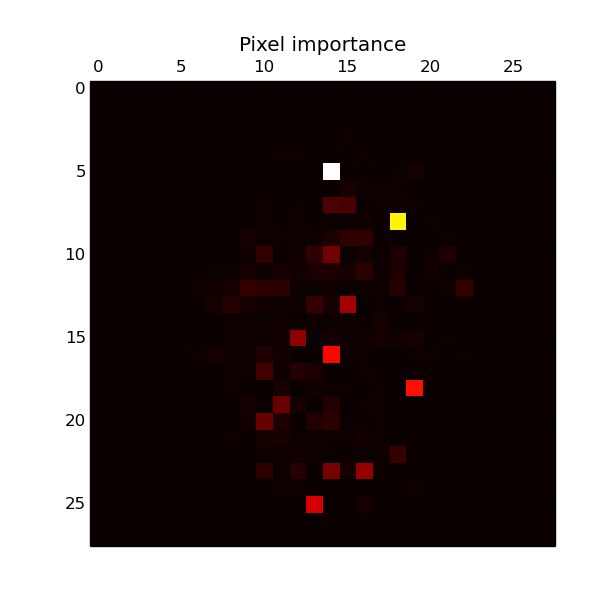
\includegraphics[width=0.4\textwidth]{tree_importance}
      \caption{Pixel importance for fine-tuned Decision Tree classifier}
      \label{fig:tree_importance}
    \end{figure}
    \begin{figure}[!hbt]
      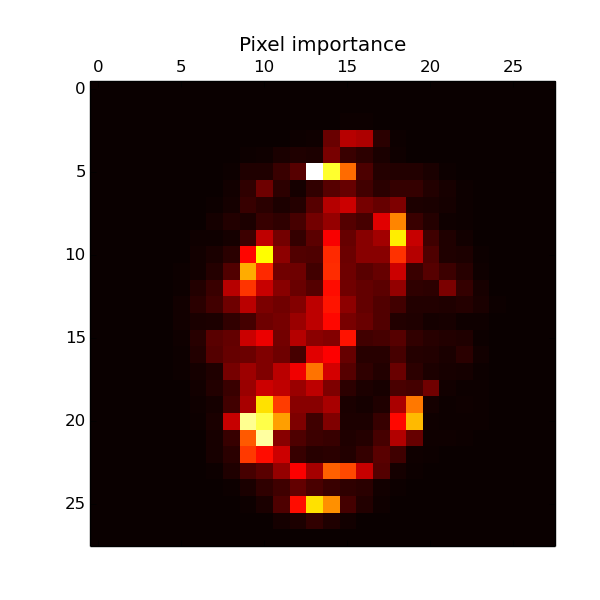
\includegraphics[width=0.4\textwidth]{random_importance}
      \caption{Pixel importance for fine-tuned Random Forest classifier}
      \label{fig:random_importance}
    \end{figure}
    
    Figures \ref{fig:tree_importance} and \ref{fig:random_importance} depict pixel importance as seen by fine-tuned Decision Tree and Random Forest classifiers respectively. It seems that due to the limited depth and number of features the individual trees of Random Forest better cover the feature space of the MNSIT dataset, allowing for improved generalization.


\begin{thebibliography}{5}

	\bibitem{MNIST}
	Y.~LeCun, L.~Bottou, Y.~Bengio, and P.~Haffner. ``Gradient-based learning applied to document recognition.'' Proceedings of the IEEE, 86(11):2278-2324, November 1998.
	
	\bibitem{VSVM}
	D.~Decoste and B.~Schölkopf. ``Training invariant support vector machines.'' Machine learning 46, no. 1-3 (2002): 161-190.

	\bibitem{MNIST_Website} % Web document
	Y.~LeCun, C.~Cortes, C.J.C.~Burges. The MNIST database of handwritten digits.
	\url{http://yann.lecun.com/exdb/mnist/}.
	
	\bibitem{UFLDL} % Web document
	A.~Ng, J,~Ngiam, C.Y.~Foo, Y.~Mai and C~Suen. ``Unsupervised Feature Learning and Deep Learning Tutorial.''
	\url{http://ufldl.stanford.edu/wiki/index.php/UFLDL_Tutorial}.

\end{thebibliography}

% Your document ends here!
\end{document}
